\section{Weapon Selection}
\label{sec:modules:controlscheme:weaponselection}

In shooter games where the player can carry more than one weapon at a time, it is important that the player is able to switch to his weapon of choice as quickly as possible. For example if the currently equipped weapon is low on ammunition and there are enemies nearby then the player will need to switch to a different weapon in order to save himself. The quicker the player can switch weapon in this case the more likely he is to be able to save himself.

In the game \texttt{Counter-Strike}\cite{counterstrike} the player can have a primary and secondary firearm, a knife, and various grenades. All of these weapons are by default bound to the number keys on the keyboard meaning the player can select his primary firearm by pressing the \texttt{1} key and his secondary firearm by pressing the \texttt{2} key. 

This works well because the player only has a few weapons available at a time. Hence he can use the number keys that are situated close to the default movement buttons (\texttt{W}, \texttt{A}, \texttt{S}, and \texttt{D}), allowing him to switch weapon while moving.

In a game like \texttt{Unreal Tournament}\cite{unrealtournament} where the player may have up to ten weapons at a time, the player may not be able to move while selecting a weapon bound to the \texttt{8} or \texttt{9} keys as they are not as close to the movement keys as the lower numbers.
Instead an option which is supported in both of these games is to use the \texttt{next} and \texttt{previous} weapon buttons. These buttons treat the list of weapons as a circular list so if the player has the first weapon equipped uses the \texttt{previous} weapon button he will equip the last weapon.

Binding weapons to number keys is not a viable option when developing a shooter game for mobile platforms, as players will not be playing with a keyboard. It would be possible to line up all the available weapons somewhere one the screen, but this would take up too much screen as the top part is already covered by the display of health, armor, and resources.

Using \texttt{previous} and \texttt{next} buttons to allow the player to switch weapons while only taking up very little screen space, but if too many weapons are available it may take too long for the player to select the desired weapon.
Instead it was decided to use a circular weapon selecion menu as show in figure \ref{fig:weaponselection} where the weapons available to the player are shown in small portions of the circle. On mobile devices the player can open up this menu by tapping on his weapon icon in the UI and select a weapon by tapping it.

\begin{figure}[H]
\centering
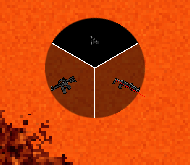
\includegraphics[width=0.5\textwidth]{figures/controlscheme/weapon_selection}
\caption{Weapon selection menu with three weapons available.}
\label{fig:weaponselection}
\end{figure}


The circle of the menu will retain its size but will be partitioned dynamically according to the amount of weapons available to best fit the weapons in the circle. This means that if there are two weapons available they will each be assigned half of the circle, where as the ones in figure \ref{fig:weaponselection} occupy a third each.

With too many weapons available this will result in a lack of space for weapons in the circle and it will be difficult for a player to select the desired weapon. Instead the idea is to have the circle contain weapon categories, eg. pistols or rifles, and then once these are selected then the contents of the circle will be replaced with weapons as in the current menu. 